%Template for the submission to:

%   The Annals of Applied Probability   [aap]
%   The Annals of Statistics            [aos] 
%   The Annals of Applied Statistics    [aoas]
%   Stochastic Systems                  [ssy]
%
%Author: In this template, the places where you need to add information
%        (or delete line) are indicated by {???}.  Mostly the information
%        required is obvious, but some explanations are given in lines starting
%Author:
%All other lines should be ignored.  After editing, there should be
%no instances of ??? after this line.

% use option [preprint] to remove info line at bottom
% journal options: aop,aap,aos,aoas,ssy
% natbib option: authoryear
\documentclass[aos,preprint]{imsart}  % use this for archive version. 

%\documentclass[aos]{imsart}  % use this for AOS submission
\setattribute{journal}{name}{} 

%\usepackage{amsthm,amsmath,natbib}
%\RequirePackage[colorlinks,citecolor=blue,urlcolor=blue]{hyperref}
% \usepackage{mdframed}
\usepackage{color}
\usepackage{enumerate}
\usepackage{amsmath,amsthm,amsfonts}
\usepackage{graphicx}
\usepackage[export]{adjustbox}
\usepackage{multirow}
\usepackage{hyperref}
\usepackage{extarrows}
%\usepackage[longnamesfirst]{natbib}
%\usepackage{multirow}
\usepackage{algorithm, algpseudocode}
\usepackage{soul}
\usepackage{MnSymbol}
\usepackage{natbib}
% provide arXiv number if available:
%\arxiv{arXiv:0000.0000}
\newcommand{\ignore}[1]{}
% put your definitions there:
\startlocaldefs


\numberwithin{table}{section} % together with amsmath
\renewcommand{\algorithmiccomment}[1]{\hspace{2em}// #1} 
\renewcommand{\algorithmicrequire}{\textbf{Input:}}
\renewcommand{\algorithmicensure}{\textbf{Output:}}
\theoremstyle{plain}
\newtheorem*{assum*}{Assumption}
\theoremstyle{plain}
\newtheorem{thm}{Theorem}%[section]
\newtheorem{lem}[thm]{Lemma}%[section]
\newtheorem{ex}{Example}
\newtheorem{cor}[thm]{Corollary}
\newtheorem{defn}{Definition}[section]
\newtheorem{assum}{Assumption}
%\newtheorem{claim}[lem]{}

\makeatletter
\newenvironment{subenvir}[1]{%
	\def\subtheoremcounter{#1}%
	\refstepcounter{#1}%
	\protected@edef\theparentnumber{\csname the#1\endcsname}%
	\setcounter{parentnumber}{\value{#1}}%
	\setcounter{#1}{0}%
	\expandafter\def\csname the#1\endcsname{\theparentnumber.\Alph{#1}}%
	\ignorespaces
}{%
	\setcounter{\subtheoremcounter}{\value{parentnumber}}%
	\ignorespacesafterend
}
\makeatother
\newcounter{parentnumber}

\newtheoremstyle{TheoremNum}
{\topsep}{\topsep}              %%% space between body and thm
{\itshape}                      %%% Thm body font
{}                              %%% Indent amount (empty = no indent)
{\bfseries}                     %%% Thm head font
{.}                             %%% Punctuation after thm head
{ }                             %%% Space after thm head
{\thmname{#1}\thmnote{ \bfseries #3}}%%% Thm head spec




\theoremstyle{TheoremNum}



\newtheorem{thm_old}{Theorem}
\newtheorem{cor_old}{Corollary}
\newtheorem{lem_old}{Lemma}
%%----------------------------
%\theoremstyle{numberplain}
%\newtheorem{thm}{\bf Theorem}





%---------------
%\theoremstyle{nonumberplain} % does not work
%\theoremsymbol{$\diamondsuit$}
\newtheorem*{ans}{Answer}
\newtheorem*{rem}{\bf Remark}


\newcommand {\Reals}  {{\rm I \! R}}
\newcommand {\Naturals}  {{\rm I \! N}}
\newcommand {\reals}  {{\rm I \! R}}
\newcommand {\Rationals}  {{\rm I \! Q}}
\newcommand {\Integers}  {{\rm I \! Z}}

\newcommand {\Procrustes}  {{\cP\cT}}
\newcommand{\tY}{{\hat{Y}}}

\newcommand{\1}{{\bf 1}}

\newcommand{\bbA}{\mathbb{A}}
\newcommand{\bbB}{\mathbb{B}}
\newcommand{\bbD}{\mathbb{D}}
\newcommand{\bbE}{\mathbb{E}}
\newcommand{\bbK}{\mathbb{K}}
\newcommand{\bbH}{\mathbb{H}}
\newcommand{\bbI}{\mathbb{I}}
\newcommand{\bbG}{{\mathbb{G}}}
\newcommand{\bbL}{{\mathbb{L}}}
\newcommand{\bbM}{{\mathbb{M}}}
\newcommand{\bbN}{{\mathbb{N}}}
\newcommand{\bbO}{{\mathbb{O}}}
\newcommand{\bbP}{\mathbb{P}}
\newcommand{\bbQ}{\mathbb{Q}}
\newcommand{\bbR}{\mathbb{R}}
\newcommand{\bbS}{{\mathbb{S}}}
\newcommand{\bbT}{\mathbb{T}}
\newcommand{\bbU}{\mathbb{U}}
\newcommand{\tbU}{{\mathbb{\tilde  U}}}
\newcommand{\bbV}{\mathbb{V}}
\newcommand{\bbW}{{\mathbb{W}}}
\newcommand{\bbX}{{\mathbb{X}}}
\newcommand{\bbY}{{\mathbb{Y}}}
\newcommand{\bbZ}{\mathbb{Z}}

\newcommand{\hbeta}{{\hat{\beta}}}
\newcommand{\srhbeta}{{\hat{\beta}^{SR}}}
\newcommand{\uhbeta}{{\hat{\beta}^{u}}}
\newcommand{\aghbeta}{{\hat{\beta}}}
\newcommand{\naY}{{\hat{Y}^{GaG}}}
\newcommand{\srhsig}{{\hat{\sigma}^{SR}}}

\newcommand{\expc}{{\E}}

\newcommand{\cA}{\mathcal{A}}
\newcommand{\cB}{\mathcal{B}}
\newcommand{\cC}{\mathcal{C}}
\newcommand{\cD}{\mathcal{D}}
\newcommand{\cF}{\mathcal{F}}
\newcommand{\cG}{\mathcal{G}}
\newcommand{\cK}{\mathcal{K}}
\newcommand{\cM}{\mathcal{M}}
\newcommand{\cL}{\mathcal{L}}
\newcommand{\cS}{\mathcal{S}}
\newcommand{\cT}{\mathcal{T}}
\newcommand{\cU}{\mathcal{U}}
\newcommand{\cV}{\mathcal{V}}
\newcommand{\cW}{\mathcal{W}}
\newcommand{\cX}{\mathcal{X}}
\newcommand{\Ra}{{\mathcal{R}}}
\newcommand{\Null}{{\mathcal{N}}}
\newcommand{\Range}{{\mathcal{R}}}

\newcommand{\0}{{\vec{\mathbf{0}}}}
\renewcommand{\a}{{\mathbf{a}}}
\renewcommand{\b}{{\mathbf{b}}}
\newcommand{\e}{{\mathbf{e}}}
\newcommand{\f}{{\mathbf{f}}}
\renewcommand{\i}{{\mathbf{i}}}
\newcommand{\m}{{\mathbf{m}}}
\renewcommand{\r}{{\mathbf{r}}}
\newcommand{\s}{{\mathbf{s}}}
%\renewcommand{\t}{{\mathbf{t}}}
\renewcommand{\u}{{\mathbf{u}}}
\renewcommand{\v}{{\mathbf{v}}}
\newcommand{\w}{{\mathbf{w}}}
\newcommand{\x}{{\mathbf{x}}}
\newcommand{\y}{{\mathbf{y}}}
\newcommand{\yhat}{{\mathbf{\hat{y}}}}
\newcommand{\z}{{\mathbf{z}}}
\newcommand{\A}{{\mathbf{A}}}
\newcommand{\B}{{\mathbf{B}}}
%\newcommand{\C}{{\mathbf{C}}}
\newcommand{\D}{{\mathbf{D}}}
\renewcommand{\H}{{\mathbf{H}}}
\newcommand{\I}{{\mathbf{I}}}
\newcommand{\M}{{\mathbf{M}}}

\newcommand{\N}{{\mathbf{N}}}

\newcommand{\E}{{\mathbf{E}}}
\renewcommand{\P}{{\mathbf{P}}}
\newcommand{\Q}{{\mathbf{Q}}}
\newcommand{\R}{{\mathbf{R}}}
\renewcommand{\S}{{\mathbf{S}}}
\newcommand{\T}{{\mathbf{T}}}
%\renewcommand{\U}{{\mathbf{U}}}
\newcommand{\V}{{\rm V}}
\newcommand{\Var}{{\rm Var}}
\newcommand{\W}{{\mathbf{W}}}
\newcommand{\X}{{\mathbf{X}}}
\newcommand{\Y}{{\mathbf{Y}}}
\newcommand{\Z}{{\mathbf{Z}}}
\newcommand{\betahat} {{b}}   % could be {{\hat{\beta}}}

\makeatletter
\newcommand{\doublewidetilde}[1]{{%
		\mathpalette\double@widetilde{#1}%
}}
\newcommand{\double@widetilde}[2]{%
	\sbox\z@{$\m@th#1\widetilde{#2}$}%
	\ht\z@=.9\ht\z@
	\widetilde{\box\z@}%
}
\makeatother
\newcommand{\tm}{{\tilde m } }
\newcommand{\tp}{{\tilde p } }
\newcommand{\ttp}{\doublewidetilde{p}}

\newcommand{\bX}{{\mathbf{\bar{X}}}}
\newcommand{\by}{{\mathbf{\bar{y}}}}

\newcommand{\cN}{{\cal N}}
\newcommand{\cO}{{\cal O}}
\newcommand{\cP}{{\cal P}}
\newcommand{\cQ}{{\cal Q}}
\newcommand{\cR}{{\cal R}}

\newcommand{\diag}{{\rm diag}}
\newcommand{\Prob}{{\P}}
\newcommand{\tr}{{\rm tr}}
\newcommand{\var}{{\rm var}}
\newcommand{\DiaEig}{{ \Sigma }}
\newcommand{\rank}{{ rank }}

\newcommand{\dps}{\displaystyle}
%%----------------------------
\endlocaldefs


\numberwithin{equation}{section}

\begin{document}
\title{Blotto-game competition from Jane Street}

\author{Yezheng Li, \today}	


\begin{abstract}ABSTRACT:
	
\textbf{What is your entry?}
	
	In Blotto-game competition from Jane Street, I propose my entry as the following: if I have $n_A$ soliders, I may assign to each castle in the way shown in the table \ref{tab:my entry}.
	
\textbf{How did you go about coming up with it?}

See details in section \ref{sec:implementations of other's research work}. After theoretically understand algorithms \citep{ahmadinejad2016duels,behnezhad2017faster,vu2018efficient}, I impliment two two-step algorithms in \citep{behnezhad2017faster,vu2018efficient}. The two algorithms are different from each other only in the first step of  generating mixed-strategy Nash equilibriums \citep{li2018blotto}. After comparision of entry candidates, my proposed entry candidates are from  \citep{behnezhad2017faster} and are summarized in table \ref{tab:my entry}. 

\textbf{How would your entry change if your were only allowed 90 soliders? What about if your received 110 soldiers? (In both cases every one else still gets 100)}

See table \ref{tab:my entry} and see section \ref{sec:implementations of other's research work} where general procedures are implemented.
\end{abstract}
\tableofcontents
\maketitle
	\begin{table}[htbp] \caption{My entries depending on $n_A$, the number of soldiers I have.}
	\label{tab:my entry}
	\begin{center}
		\begin{tabular}{|c|c|c|c|c|c|c|c|c|c|c|} \hline  
			$n_A$/castle point $v_i$ & 1 & 2 & 3 & 4 & 5 & 6 & 7 & 8 & 9 & 10 \\\hline
			100 & 0 & 3 & 8 & 12 & 17 & 22 & 27 & 11 & 0 & 0 \\
			90 & 0 & 4 & 8 & 12 & 16 & 22 & 26 &2  &  0 & 0 \\
			110 & 0 & 4 & 9 & 14 & 19 & 23 & 28 & 3 & 1 & 9 
			\\ \hline				
		\end{tabular}
	\end{center}
	
\end{table}
\section{Introduction}
We formulate general  "N-dimensional asymmetric hetergenous Blotto game" partially referring to \citep{schwartz2014heterogeneous}. 

We are given $\v \in\Reals_{+}^{N}$, an $N$ dimensional vector as points for $N$ castles, $n_A$, $n_B$ as two postive integers, representing number of soliders owned by $A$ (me) and $B$ (rival), respectively. 
$$\x^A \in [n_A]^N, \x^B \in [n_B]^N, \1_N^T\x^A =n_A, \1_N^T\x^B =n_B, $$ are partitions of $n_A,n_B$ respectively where $[M] \triangleq\{0,1,\ldots, M\}$ for a positive integer $M$.

For  $\x^B$ fixed, the pure strategy of finding $\x^A$ is 
\begin{equation}
\max_{\x^A \in [n_A]^N,  \1_N^T\x^A =n_A} g\left( \x^A, \x^B\right) \triangleq \sum_{i = 1}^N v_i sgn\left( \x^A_i -  \x^B_i\right),
\end{equation}
where $sgn(x) \triangleq \left\{ \begin{array}{cc}
1, & x>0; \\ 0, & x = 0;\\ -1, & x<0.
\end{array} \right.$.

\subsection{Mixed strategy Nash equilibrium}
One relaxation is to study continous Blotto games where they have $\x^A, \x^B \in \Reals_{\ge 0}^N$ instead of $\x^A \in [n_A]^N, \x^B \in [n_B]^N$ \citep{gross1950continuous,laslier2002two,thomas2018n}. Since \citep{gross1950continuous,laslier2002two,thomas2018n} imply there is no pure-strategy Nash equilibrium with our $\v = [1,2,\ldots, N]^T, N=10$, mixed strategy Nash equilibrium is one focus of attention.

Mixed strategy Nash equilibrium is a useful concept and is essentially the first of the two-step procedure that we will mention in section \ref{sec:implementations of other's research work}. However, we stick to discrete version \citep{ahmadinejad2016duels,behnezhad2017faster,vu2018efficient} although it is possible to come up with entry candidates from solutions to continuous Blotto games. 
\section{Implementations of two  research work}
\label{sec:implementations of other's research work}
Besides investigation into theoretical work \citep{thomas2018n,roberson2006colonel,hart2008discrete,hortala2012pure}, this solution implements Python version of \citep{vu2018efficient} and Julia version of \citep{behnezhad2017faster}. Codes are updated on \citep{li2018blotto}.


\subsection{Two-step procedure}

We can use the two-step procedure in \citep{vu2018efficient} to summarize our two-step procedure, since \citep{behnezhad2017faster} (as an improvement of \citep{ahmadinejad2016duels}) is just an alternative to algorithm I (DIU strategy) in \cite{vu2018efficient}.

First step is to generate mixed-strategy Nash equilibrium and is essentially the difference between two research works (that is, two algorithms I used to generate my entry candidates).  \citep{vu2018efficient} uses its DIU strategy where the idea essentially originates from the uniform marginal distribution proved in \citep{gross1950continuous,laslier2002two}. \citep{behnezhad2017faster} solves an improved LP (relative to \citep{ahmadinejad2016duels}) and actually has no randomness.

Second step is a minor adjustment to algorithm II in \citep{vu2018efficient}. The necessary adjustment is to have marginal distribution $G_i(j-1)$ instead of $G_i(j)$ in fourth line of the pseudocode since if $x_i^A= x_i^B$, we assign  reward to neither player $A$ nor player $B$, while \citep{behnezhad2017faster} has its corresponding "$\alpha$-tie-breaking rule". This second step corresponds to \textit{best\_response.py} in \citep{li2018blotto}.
\subsection{Entry candidates}
While \citep{vu2018efficient} has randomness due to sampling in DIU strategy (algorithm I in \citep{vu2018efficient}), Julia version of \citep{behnezhad2017faster} solves a LP and actually has no randomness. At a glimpse, a selection of entry candidates are recorded in \textit{document.csv} and are shown in figure \ref{fig:Results document.csv where yellows are for }; by "selection", I mean I definitely can generate more; here the paper is just for demonstration.


Now let's compare the entry candidates. Comparision in \citep{vu2018efficient} does not focus on our scenario, but emphasizing the cases when $N$, the number of battles is large. In addition to the fact that \citep{behnezhad2017faster} has more theoretical guarantee than \citep{vu2018efficient}'s strategy, there is one simple way to heuristically show that \citep{behnezhad2017faster} is better: with the candidates in figure \ref{fig:Results document.csv where yellows are for }, we do head-to-head tournaments. It is obviously meaningful for $n_A=100$; to be honest, for $n_A=90, 110$, the tournaments are less intepretable since the mixed strategy Nash equilibriums are found in games with rival $n_B= 100$. Whatever the case, I show three tournaments in figure \ref{fig:output table 100}, \ref{fig:output table 90}, \ref{fig:output table 110}. One can immediately realize "Julia"  in last two rows (the two are identical in figure \ref{fig:Results document.csv where yellows are for } and showing two rows is just one of the ways to double check my analysis and codes all the way), win the most. As a result, we fill table \ref{tab:my entry} by \citep{behnezhad2017faster}'s simulation.


\section{Conclusion}

After theoretically understand algorithms \citep{ahmadinejad2016duels,behnezhad2017faster,vu2018efficient}, I impliment two two-step algorithms in \citep{behnezhad2017faster,vu2018efficient}. The two algorithms are different from each other only in the first step of  generating mixed-strategy Nash equilibriums \citep{li2018blotto}. After comparision of entry candidates, my proposed entry candidates are from  \citep{behnezhad2017faster} and are summarized in table \ref{tab:my entry}. 
\begin{figure}[ht]
	\caption{Selected results (by "selected", I mean I definitely can generate more; here the paper is just for demonstration) in \textit{document.csv} where yellows are for $n_A=100$, greens are for $n_A=90$ and orange are for $n_A =110$. Column names include "number of DIUs" as well as "number of castles", "rival's soldiers", "my soliders" that are literally understandable. "number of DIUs" has attribution values of the following (1) numbers, indicating number of simulations of DIU in \citep{vu2018efficient} or (2) "Julia" indicating the mixed strategy Nash equilibrium is generated from \cite{behnezhad2017faster}.}
	\label{fig:Results document.csv where yellows are for }
	\begin{center}
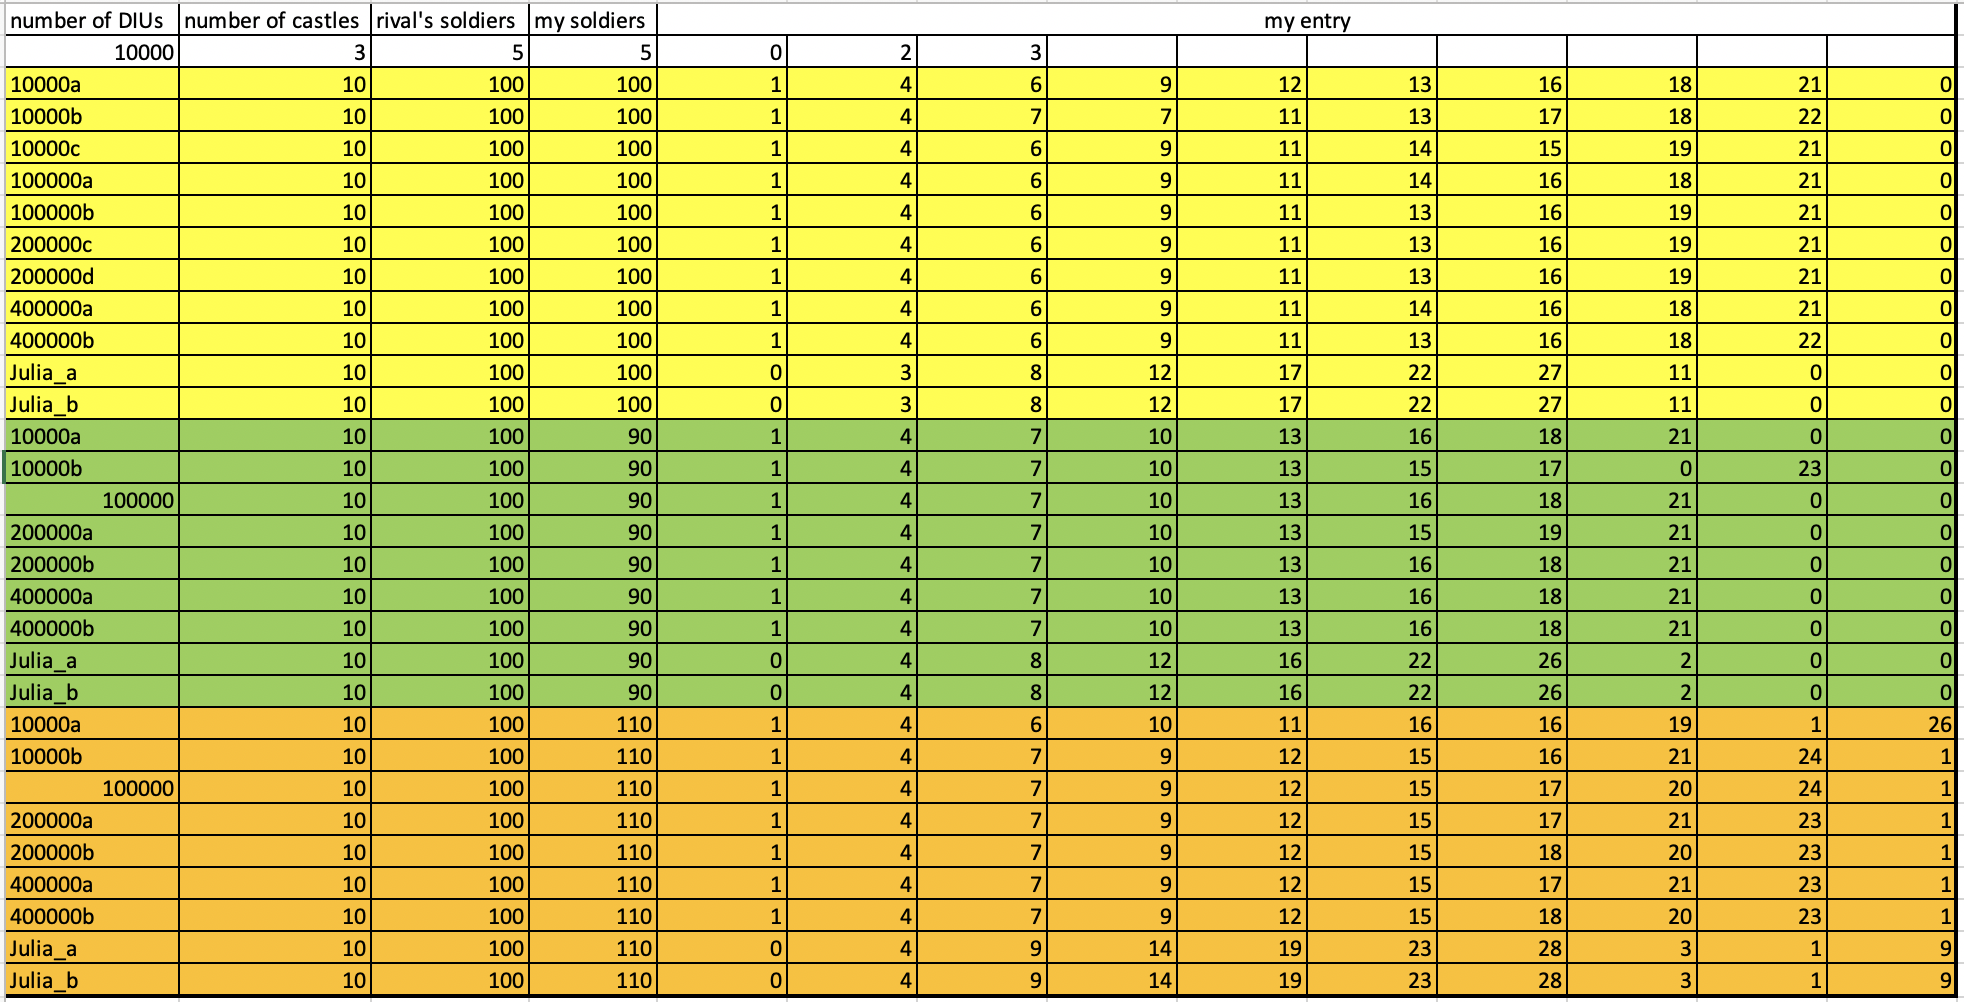
\includegraphics[width =\textwidth]{solutions.png}
	\end{center}
	
\end{figure}
\begin{figure}[ht]
	\caption{Pairwise results in the tournament of yellow entry candidates from \textit{document.csv} where $n_A=100$. Each row represents my entry while each column represents the rival's. Correponding entry assignments are in figure \ref{fig:Results document.csv where yellows are for }.}
	\label{fig:output table 100}
	\begin{center}
		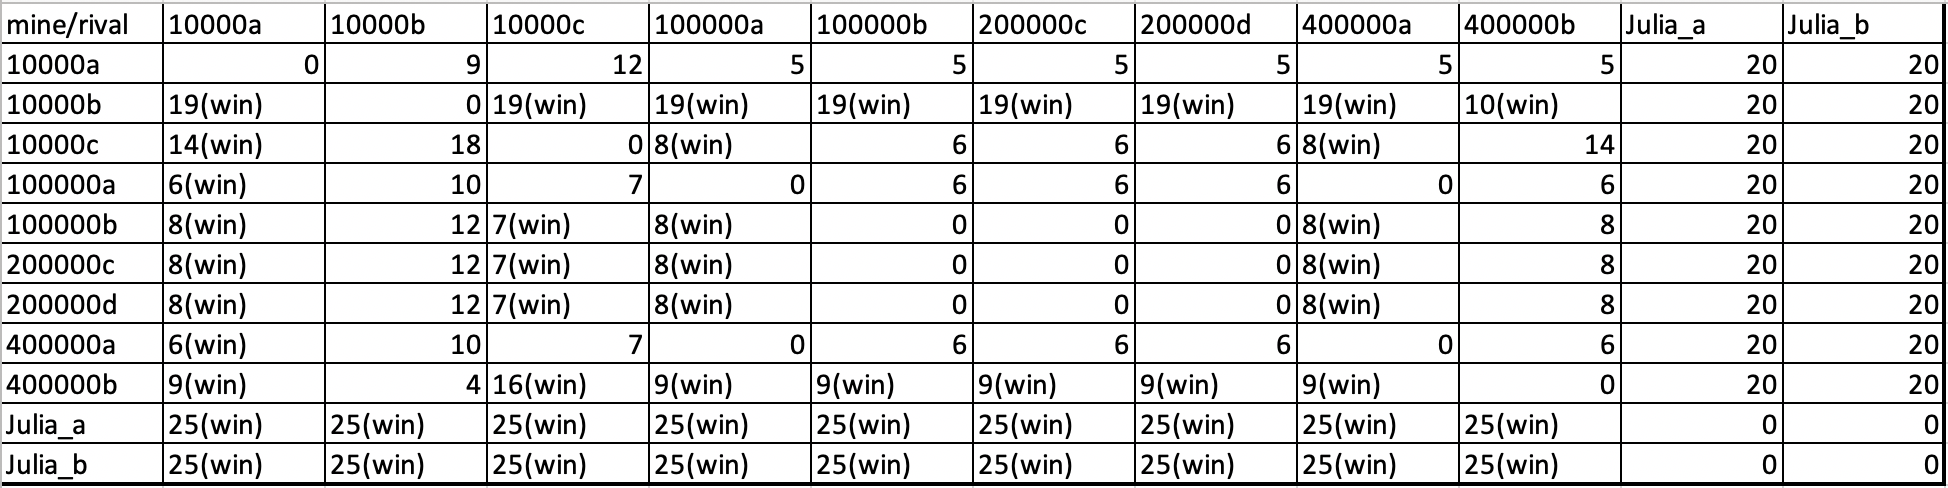
\includegraphics[width =\textwidth]{output_table_100.png}
	\end{center}
	
\end{figure}

\begin{figure}[ht]
	\caption{Pairwise results in the tournament of yellow entry candidates from \textit{document.csv} where $n_A=90$. Each row represents my entry while each column represents the rival's. Correponding entry assignments are in figure \ref{fig:Results document.csv where yellows are for }.}
	\label{fig:output table 90}
	\begin{center}
		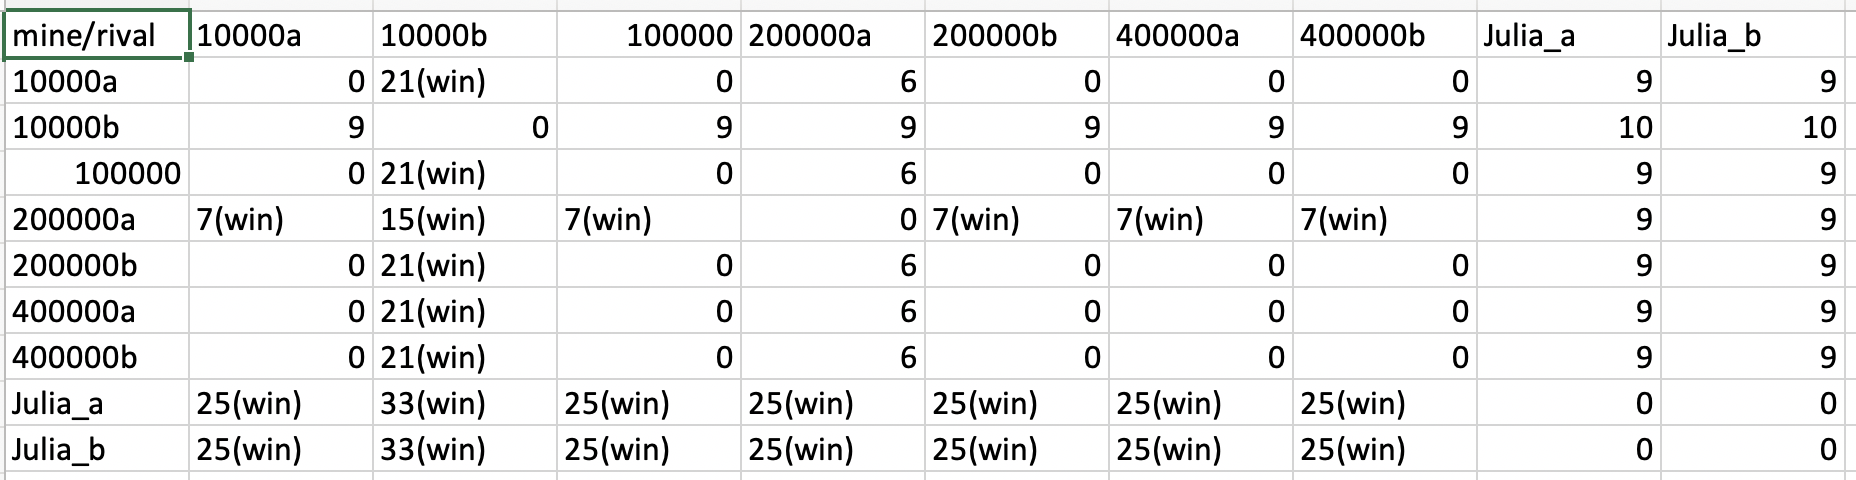
\includegraphics[width =\textwidth]{output_table_90.png}
	\end{center}
	
\end{figure}

\begin{figure}[ht]
	\caption{Pairwise results in the tournament of yellow entry candidates from \textit{document.csv} where $n_A=110$. Each row represents my entry while each column represents the rival's. Correponding entry assignments are in figure \ref{fig:Results document.csv where yellows are for }.}
	\label{fig:output table 110}
	\begin{center}
		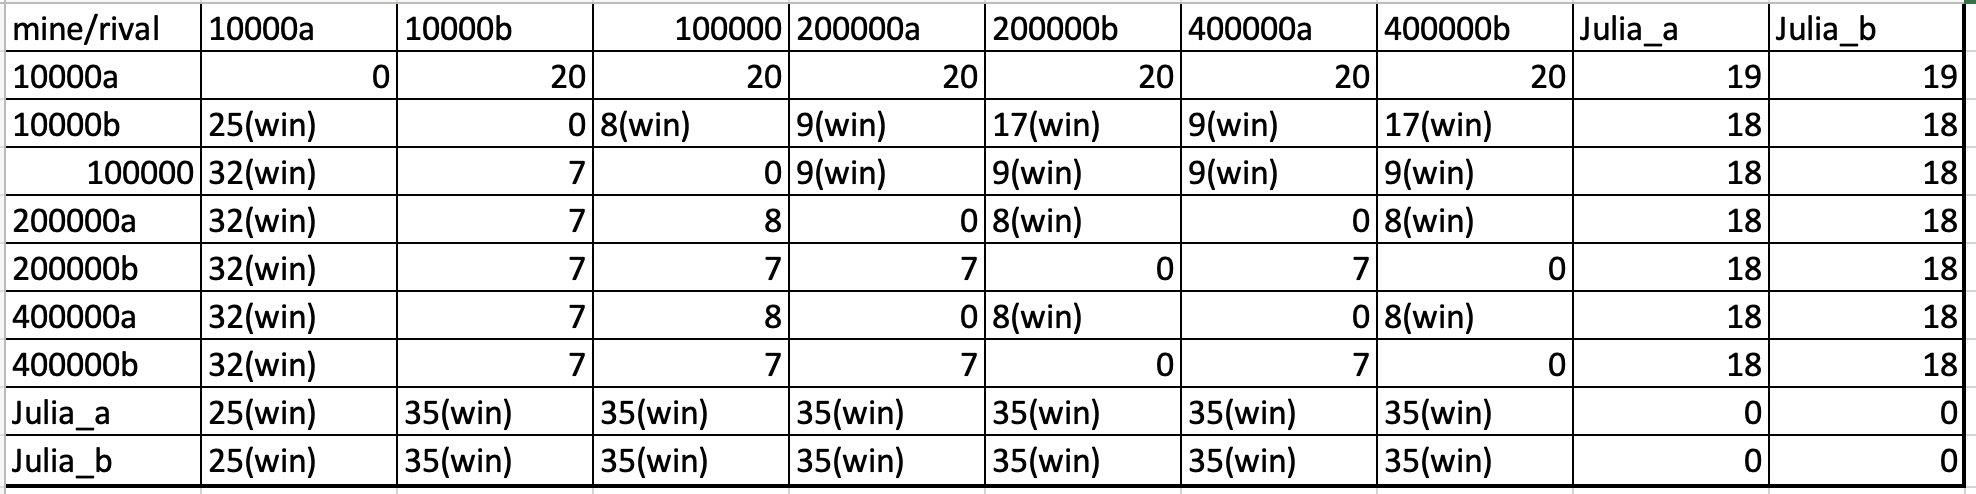
\includegraphics[width =\textwidth]{output_table_110.png}
	\end{center}
	
\end{figure}


%\bibliographystyle{imssart-nameyear}
\bibliographystyle{apalike}
%\bibliographystyle{jtbnew}%{decsci}
\bibliography{statistics}
\end{document}
